\documentclass[12pt,a4paper]{article}
\usepackage{amssymb}
\usepackage{graphicx}
\pagestyle{empty}
\textwidth = 15.5 cm
\textheight = 23.5 cm
\topmargin =-1.0 cm
\oddsidemargin = 0.5 cm
\listparindent=0pt
\itemsep=5pt
\def\r{{\bf r}}
\begin{document} 
\title{Notes on pseudopotential generation}
\author{\em Paolo Giannozzi\\
Universit\`a di Udine and IOM-Democritos, Trieste\\
URL: {\tt http://www.fisica.uniud.it/$\thicksim$giannozz}}
\maketitle
\date
\section{Introduction} 

When I started to do my first first-principle calculation
(that is, my first$^2$-principle calculation) with Stefano Baroni
on CsI under pressure (1985), it became quickly evident that
available pseudopotentials (PP's) couldn't do the job. So we 
generated our own PP's. Since that first experience I have 
generated a large number of PP's and people keep asking me 
new PP's from time to time. I am happy that "my" PP's are 
appreciated and used by other people. I don't think however 
that the generation of PP's is such a hard task that it requires 
an official (or unofficial) PP wizard to do this. For this reason 
I want to share here my (little) experience.

These notes are written in general but having in mind the capabilities of
the {\tt atomic} package, included in the {\sc Quantum ESPRESSO} distribution 
(\texttt{http://www.quantum-espresso.org}). {\tt atomic}, mostly written
and maintained by Andrea Dal Corso, is the evolution of an older generation 
code I maintained for several years. {\tt atomic} can generate both 
Norm-Conserving (NC) \cite{NC} and Ultrasoft (US) \cite{van} PP's,
plus Projector Augmented Waves (PAW) \cite{PAW} sets.
It allows multiple projectors, full relativistic calculations,
spin-split PP's for spin-orbit calculations.
For the complete description of the input of \texttt{atomic},
please refer to files \texttt{INPUT\_LD1.txt} and 
\texttt{INPUT\_LD1.html}.

\subsection{Who needs to generate a pseudopotential?}

There are at least three well-known published sets of NC-PP's:
those of Bachelet, Hamann, and Schl\"uter \cite{BHS},
those of Gonze, Stumpf, and Scheffler \cite{Gonze}, and
those of Goedecker, Teter, and Hutter \cite{Goedecker}. 
Moreover, all major packages for electronic-structure calculations
include a downloadable table of PP's. One could then wonder 
what a PP generation code is useful for. The problem is that 
sometimes available PP's will not suit your needs. For instance,
you may want:
\begin{enumerate}
 \item[--] a better accuracy;
 \item[--] PP's generated with some exotic or new exchange-correlation
     functional;
 \item[--] a different partition of electrons into valence and core;
 \item[--] ``softer'' PP's (i.e. PP that require a smaller cutoff
           in plane-wave calculations);
 \item[--] PP's with a core-hole for calculations of X-ray Adsorption
           Spectra;
 \item[--] all-electron wavefunctions reconstruction (requires the
           knowledge of atomic all-electron and pseudo-orbitals used in
           the generation of PP's);
\end{enumerate}
or you may simply want to know what is a PP, how to produce PP's, 
how reliable they are.

\subsection{About similar work}

There are other PP generation packages available on-line.
Those I am aware of include:
\begin{itemize}
\item the code by Jos\'e-Lu{\'\i}s Martins {\em et al.}\cite{TM}:\\
{\tt http://bohr.inesc-mn.pt/\~{}jlm/pseudo.html}
\item the {\tt fhi98PP} package\cite{fhi98PP}:\\
{\tt http://www.fhi-berlin.mpg.de/th/fhi98md/fhi98PP}
\item the OPIUM code by Andrew Rappe {\em et al.}\cite{RRKJ}:\\
{\tt http://opium.sourceforge.net/}
\item David Vanderbilt's US-PP package \cite{van}:\\
{\tt http://www.physics.rutgers.edu/\~{}dhv/uspp/index.html}.
\end{itemize}
Other codes may be available upon request from the authors.

Years ago, it occurred to me that a web-based PP generation
tool would have been nice. Being too lazy and too ignorant 
in web-based applications, I did nothing.
I recently discovered that Miguel Marques {\em et al.} have
implemented something like this: see
{\tt http://www.tddft.org/programs/octopus/pseudo.php}.

\section{Pseudopotential generation, in general} 

In the following I am assuming that the basic PP theory 
is known to the reader. Otherwise, see 
Refs.\cite{NC,BHS,TM,fhi98PP,RRKJ} and references quoted 
therein for NC-PP's; Refs.\cite{van,PAW} for US-PP's and PAWsets. 
I am also assuming that the generated PP's are to be used
in separable form \cite{KB} with a plane-wave (PW) basis set.

The PP generation is a three-step process. First, one generates
atomic levels and orbitals with Density-functional theory (DFT). 
Second, from atomic results one generates the PP. Third, one checks 
whether the reesulting PP is actually working. If not, one tries again in 
a different way.

The first step is invariably done assuming a spherically symmetric
self-consistent Hamiltonian, so that all elementary quantum mechanics 
results for the atom apply. The atomic state is defined by the
"electronic configuration", one-electron states are defined by a
principal quantum number and by the angular momentum and are obtained
by solving a self-consistent radial Schr\"odinger-like (Kohn-Sham)
equation.

The second step exists in many variants. One can generate ``traditional'' 
single-projector NC-PP's; multiple-projector NC-PP's; or US-PP's.
The crucial step is in all cases the generation of smooth
``pseudo-orbitals''  from atomic all-electron (AE) orbitals. 
Two popular pseudization
methods are presently implemented: Troullier-Martins \cite{TM}
and Rappe-Rabe-Kaxiras-Joannopoulos \cite{RRKJ} (RRKJ).

The third step is closer to cooking than to science. There is a
large arbitrariness in the preceding step that one would like to 
exploit in order to get the "best" PP, but there is no well-defined
way to do this. Moreover one is often forced to strike a compromise
between transferability (thus accuracy) and hardness (i.e. computer 
time). This last step is the main focus of these notes.

\section{Step-by-step Pseudopotential generation} 

If you want to generate a PP for a given atom, the checklist is the
following:

\begin{itemize}
\item choose the generation parameters:
\begin{enumerate}
\item exchange-correlation functional
\item valence-core partition
\item electronic reference configuration
\item nonlinear core correction
\item type of pseudization
\item pseudization energies 
\item pseudization radii
\item local potential
\end{enumerate}
\item generate the pseudopotential
\item check for transferability
\end{itemize}
In case of trouble or of unsatisfactory results, one has to 
go back to the first step and change the generation parameters,
usually in the last four items.

\subsection{Choosing the generation parameters}

\subsubsection{Exchange-correlation functional}
\label{XC}
PP's must be generated with the {\em same} exchange-correlation
(XC) functional that will
be later used in calculations. The use of, for instance, a
GGA (Generalized Gradient Approximation) functional tegether
with PP's generated with Local-Density Approximation (LDA) 
is inconsistent. This is why the PP file contains information 
on the DFT level used in their generation: if you or your code 
ignore it, you do it at your own risk.

The \texttt{atomic} package allows PP generation for a large number of 
functionals, both LDA and GGA. Most of them have 
been extensively tested, but beware: some exotic or seldom-used functionals 
might contain bugs. Currently, \texttt{atomic} does not allow PP generation
with meta-GGA (TPSS) or hybrid functionals. For the former, an old version 
of \texttt{atomic}, modified by Xiaofei Wang, is available. 
Work is in progress for the latter.

Some functionals may present numerical problems
when the charge density goes to zero. For instance, the Becke
gradient correction to the exchange may diverge for 
$\rho \rightarrow 0$. This does not happen in a free atom
if the charge density behaves as it should, that is, as
$\rho(r)\rightarrow exp(-\alpha r)$ for $r \rightarrow \infty$.
In a pseudoatom, however, a weird behavior may arise 
around the core region, $r\rightarrow 0$, because the 
pseudocharge in that region is very small or sometimes 
vanishing (if there are no filled $s$ states). As a consequence,
nasty-looking ``spikes'' appear in the unscreened pseudopotential
very close to the nucleus. This is not nice at all but it is
usually harmless, because the interested region is really 
very small. However in some unfortunate cases there can be 
convergence problems. If you do not want to see those horrible 
spikes, or if you experience problems, you have the following
choices:
\begin{enumerate}
\item[--] Use a better-behaved GGA, such as PBE
\item[--] Use the nonlinear core correction, which ensures
          the presence of some charge close to the nucleus.
\end{enumerate}
A further possibility would be to cut the gradient correction for small 
$r$ (it used to be implemented, but it isn't any longer).
% (set variable {\tt rcut} to $\sim 0.001$ or so).

\subsubsection{Valence-core partition}
\label{ValCore}
This seems to be a trivial step, and often it is: valence states 
are those that contribute to bonding, core states are those that 
do not contribute. Things may sometimes be more complicated than 
this. For instance:
\begin{enumerate}
\item[--] in transition metals, whose typical outer electronic
configuration is something like ($n=$ main quantum number)
$nd^i(n+1)s^j(n+1)p^k$, it is not
always evident that the $ns$ and $np$ states (``semicore states'')
can be safely put into the core. The problem is that $nd$ states 
are localized in the same spatial region as $ns$ and $np$ states, 
deeper than $(n+1)s$ and $(n+1)p$ states. This may lead to poor 
transferability. Typically, PP's with semicore states in the core 
work well in solids with weak or metallic bonding, but perform poorly 
in compounds with a stronger (chemical) type of bonding.
\item[--] Heavy alkali metals (Rb, Cs, maybe also K) have a large
polarizable core. PP's with just one electron may not always give
satisfactory results.
\item[--] In some II-VI and III-V semiconductors, such as ZnSe and
GaN, the contribution of the $d$ states of the cation to the bonding 
is not negligible and may require explicit inclusion of those $d$ 
states into the valence.
\end{enumerate}
In all these cases, promoting the highest core states $ns$ and $np$,
or $nd$, into valence may be a computationally
expensive but obliged way to improve poor transferability. . 

You should include semicore states into valence only if really needed:
their inclusion in fact makes your PP harder (unless you resort to 
US pseudization) and increases the number of electrons. In principle 
you should also use more than one projector per angular momentum, 
because the energy range to be covered by the PP with semicore electrons 
is much wider than without. If you don't, the transferability of your PP 
may suffer (a typical phenomenon:
the error on the lattice parameter of a simple metal gets worse).

\subsubsection{Electronic reference configuration}
\label{RefConf}
This may be any reasonable configuration not too far away from
the expected configuration in solids or molecules. As a first
choice, use the atomic ground state, unless you have a reason 
to do otherwise, such as for instance:
\begin{enumerate}
\item[--]
   You do not want to deal with unbound states.
   Very often states with highest angular momentum $l$ are not bound
   in the atom (an example: the $3d$ state in Si is not bound on the
   ground state $3s^23p^2$, at least with LDA or GGA). In such a case 
   one has the choice between 
   \begin{enumerate} 
      \item[--] using one configuration for $s$ and $p$, another, more
                ionic one, for $d$, as in Refs.\cite{BHS,Gonze};
      \item[--] choosing a single, more ionic configuration for which 
                all desired states are bound;
      \item[--] generate PP's on unbound states: requires to choose
                a suitable reference energy.
   \end{enumerate}
\item[--]
   The results of your PP are very sensitive to the chosen configuration.
   This is something that in principle should not happen, but
   I am aware of at least one case in which it does. In III-V
   zincblende semiconductors, the equilibrium lattice parameter
   is rather sensitive to the form of the $d$ potential of the 
   cation (due to the presence of $p-d$ coupling between anion 
   $p$ states and cation $d$ states \cite{Zunger}). By varying
   the reference configuration, one can change the equilibrium 
   lattice parameter by as much as $1-2\%$. 
   The problem arises if you want to calculate accurate dynamical
   properties of GaAs/AlAs alloys and superlattices: you need to
   get a good theoretical lattice matching between GaAs and AlAs,
   or otherwise unpleasant spurious effects may arise. When I was 
   confronted with this problem, I didn't find any better solution
   than to tweak the $4d$ reference configuration for Ga until I got
   the observed lattice-matching.
\item[--]
   You know that for the system you are interested in, the atom will 
   be in a given configuration and you try to stay close to it.
   This is not very elegant but sometimes it is needed. For instance,
   in transition metals described by a PP with semicore states in the 
   core, it is probably wise to chose an electronic configuration for 
   $d$ states that is close to what you expect in your system (as a
   hand-waiving argument, consider that the $(n+1)s$ and $(n+1)p$ PP 
   have a hard time in reproducing the true potential if the $nd$ state,
   which is much more localized, changes a lot with respect to the
   starting configuration). In Rare-Earth compounds, leaving the $4f$ 
   electrons in the core with the correct occupancy (if known) may be 
   a quick and dirty way to avoid the well-known problems of DFT yielding 
   the wrong occupancy in highly correlated materials.
\item[--]
   You don't manage to build a decent PP with the ground state configuration, 
   for whatever reason.
\end{enumerate}

NOTE 1: you can calculate PP for a $l$ as high as you want, but you
are not obliged to use all of them in PW calculations. The general
rule is that if your atom has states up to $l=l_c$ in the core, you
need a PP with angular momenta up to $l=l_c+1$. Angular momenta
$l>l_c+1$ will feel the same potential as $l=l_c+1$, because
for all of them there is no orthogonalization to core states.
As a consequence a PP should have projectors on angular momenta up to
$l_c$; $l=l_c+1$ should be the local reference state for PW
calculations. This rule is not very strict and may be relaxed: high
angular momenta are seldom important (but be careful if they are). 
Moreover separable PP pose serious constraints on local reference $l$
(see below) and the choice is sometimes obliged. Note also that the
highest the $l$ in the PP, the more expensive the PW calculation will 
be.

NOTE 2: a completely empty configuration ($s^0p^0d^0$) or
a configuration with fractional occupation numbers are both
acceptable. Even if fractional occupation numbers do
not correspond to a physical atomic state, they correspond to a
well-defined mathematical object.

NOTE 3: PP could in principle be generated on a spin-polarized
configuration, but a spin-unpolarized one is typically used.
Since PP are constructed to be transferrable, they can describe
spin-polarized configurations as well. The nonlinear core correction
is needed if you plan to use PP in spin-polarized (magnetic)
systems.

\subsubsection{Nonlinear core correction}
\label{nlcc}
The nonlinear core correction\cite{CoreCorr} 
accounts at least partially for the nonlinearity
in the XC potential. During PP generation one first
produces a potential yielding the desired pseudo-orbitals and
pseudoenergies. In order to extract a ``bare'' PP that can be used
in a self-consistent DFT calculation, one subtracts out the screening 
(Hartree and XC) potential generated by the valence 
charge only. This introduces a trasferability error because the XC 
potential is not
linear in the charge density. With the nonlinear core correction one 
keeps a pseudized core charge to be added to the valence charge both 
at the unscreening step and when using the PP.

The nonlinear core correction {\em must} be present in one-electron PP's for
alkali atoms (especially in ionic compounds) and for PP's to be used in 
spin-polarized (magnetic) systems. It is recommended whenever there is a 
large overlap between valence and core charge: for instance, in transition 
metals if the semicore states are kept into the core. Since it is {\em never}
harmful, one can take the point of view that it should always be included,
even in cases where it will not be very useful.

The pseudized core charge used in practice is equal to the true
core charge for $r\ge r_{cc}$, differs from it  for $r < r_{cc}$
in such a way as to be much smoother. The parameter $r_{cc}$ is
typically chosen as the point at which the core charge $\rho_c(r_{cc})$ 
is twice as big as the valence charge $\rho_v(r_{cc})$. In fact the 
effect of nonlinearity is important only in regions where 
$\rho_c(r)\sim\rho_v(r)$. Alternatively, $r_{cc}$ can be provided 
in input, Note that the smaller $r_{cc}$, the more accurate the core 
correction, but also the harder the pseudized core charge, and vice versa.

\subsection{Type of pseudization}
\label{pseudization}
The \texttt{atomic} package implements two different NC pseudization 
algorithms, both claiming to yield optimally smooth PP's:
\begin{itemize}
\item Troullier-Martins \cite{TM} (TM) 
\item Rappe-Rabe-Kaxiras-Joannopoulos \cite{RRKJ} (RRKJ).
\end{itemize}
Both algorithms replace atomic orbitals in the core region 
with smooth nodeless pseudo-orbitals. The TM method uses an
exponential of a polynomial (see Appendix B); the RRKJ method 
uses three or four Bessel functions for the pseudo-orbitals in
the core region. The former is very robust. The latter may 
occasionally fail to produce the required nodeless pseudo-orbital.
If this happens, first try to force the usage of four Bessel functions
(this is achieved by setting a  small nonzero value of 
the charge density at the origin, variable \texttt{rho0}:
unfortunately it works only for $s$ states).

Second-row elements N, O, F, $3d$ transition metals, rare earths, 
are typically ``hard'' atoms, i.e. described by NC PP's requiring
a high PW cutoff. These atoms are characterized by $2p$ (N, O, F), 
$3d$ (transition metals), $4f$ (rare earths) valence states with no 
orthogonalization to core states of the same $l$ and no nodes.
In addition, as mentioned in Secs.\ref{ValCore} and \ref{RefConf}, 
there are case in which you may be forced to include semicore states
in valence, thus making the PP hard (or even harder).  
In all such cases, one should consider 
{\em ultrasoft} pseudization, unless there is a good reason to stick
to NC-PP's. For the specific case of rare earths, however, remember 
that the problem of DFT reliability preempts the (tough) problem of 
generating a PP. With US-PP's one can give up the NC requirement
and get much software PP's, at the price of introducing an augmentation 
charge that compensates for the missing charge. 

Currently, the \texttt{atomic} package generates US-PP's on top of
a ``hard'' NC-PP. In order to ensure sufficient transferability, 
at least two states per angular momentum $l$ are required. 

\subsubsection{Pseudization energies}
\label{pseudiz}
If you stick to single-projector PP's (one potential per angular momentum 
$l$, i.e. one projector per $l$ in the separable form), the choice of the 
electronic configuration automatically determines the reference states
to pseudize: for each $l$, the bound valence eigenstate is pseudized
at the corresponding eigenvalue. If no bound valence eigenstate exists,
one has to select a reference energy. The choice is rather arbitrary:
you may try something between than other valence bound state energies
and zero. 

If you have semicore states in valence, remember that for each $l$
only the state with lowest $n$ can be used to generate a single-projector
PP. The \texttt{atomic} package requires that you explicitly specify the 
configuration for unscreening in the ``test'' configuration:
see the detailed input documentation.

It is possible to generate PP's by pseudizing atomic waves,
i.e. regular solutions of the radial Kohn-Sham equation, at any
energy. More than one such atomic waves of different energy can be
pseudized for the same $l$, resulting in a PP with more than one 
projector per $l$. Note that the resulting PP is directly produced
in the separable form. 

Such possibility considerably extends the transferability, but also the 
number of ``degrees of freedom'' in the generation of a PP. As a rule of 
thumb: 
\begin{itemize}
\item start with one projector per $l$, at the energy of the bound state;
\item add a second projector at a second, higher energy not too far above 
the former. 
\end{itemize}
The latter hint seems to be counterintuitive if you have semicore states 
in valence: the obvious choice would be to include two projectors, using 
both bound states energies. Unfortunately this is currently not possible 
with the \texttt{atomic} package, because the state pseudized at the upper 
bound-state energy will necessarily have a node (in order to be orthogonal 
to the one with lower energy).

For US-PP pseudization, you should first find a suitable multi-projector 
NC-PP as above, than turn on the US-PP pseudization. This is done by
setting different NC and US pseudization radii (see Sec.\ref{radii}),

\subsubsection{Pseudization radii}
\label{radii}

For NC pseudization, one has to choose, for each state to be pseudized,
a NC pseudization radius $r_c$, at which the AE orbital and the 
corresponding NC-PP orbital match, with continuous first derivative 
at $r=r_c$. For bound states, $r_c$ is typically at the outermost peak or 
somewhat larger. The larger the $r_c$, the softer the potential 
(less PW needed in the calculations), but also the less transferable.
The $r_c$ may differ for different $l$; as a rule, one should avoid large
differences between the $r_c$'s, but this is not always possible. Also,
the $r_c$ cannot be smaller than the outermost node.

A big problem in NC-PP's is how strike a compromise between softness
and transferability, especially for difficult elements. The basic question:
``how much should I push $r_c$ outwards in order to have reasonable results 
with a reasonable PW cutoff''. has no clear-cut answer. The choice of $r_c$ 
at the outermost maximum for ``difficult'' elements (those described in 
Sec.\ref{pseudiz}): typically 0.7-0.8 a.u, even less for $4f$ electrons, 
yields very hard PP's 
(more than 100 Ry needed in practical calculations). With a little bit of 
experience one can say that for second-row ($2p$) elements, $r_c=1.1-1.2$ 
will yield reasonably good results for 50-70 Ry PW kinetic energy cutoff; 
for $3d$ transition metals, the same $r_c$ will require $> 80$ Ry cutoff
(highest $l$ have slower convergence for the same $r_c$). The above
estimates are for TM pseudization. RRKJ pseudization will yield an
estimate of the required cutoff.

For multiple-projectors NC-PP's, the $r_c$ of unbound states may be chosen 
in the same range as for bound states. If this is the first step for US-PP 
generation, use small $r_c$ and don't try to push them outwards: the
US pseudization will take care of softness. US pseudization radii can 
be chosen much larger than NC ones (e.g. 1.3$\div$ 1.5 a.u. for second-row
$2p$ elements, 1.7$\div$ 2.2 a.u. for $3d$ transition metals), but do not
forget that the sum of the $r_c$ of two atoms should not exceed the typical
bond length of those atoms.

Note that it is the hardest atom that determines the PW cutoff in a
solid or molecule. Do not waste time trying to find optimally soft 
PP's for element X if element Y is harder then element X.

\subsubsection{Choosing the local potential}

As explained in Sec. \ref{RefConf}, note 1, one needs in principle
angular momentum channels in PP's up to $l_c+1$. In the semilocal
form, the choice of a ''local'', $l$-independent potential is natural
and affects only seldom-important PW components with $l> l_c$.
In PW calculations, however, a separable, fully nonlocal form -- 
one in which the PP's is written as a local potential plus pr
ojectors -- is used.
An arbitrary function can be added to the local potential and 
subtracted to all $l$ components. Generally one exploits this 
arbitrariness to remove one $l$ component using it as local potential.
The separable form can be either obtained by the Kleinman-Bylander
projection \cite{KB} applied to single-projector PP's, or directly 
produced using Vanderbilt's procedure \cite{van} (for single-projector
PP's the two approaches are equivalent).

Unfortunately the separable form is not guaranteed to have the
correct ground state (unlike the semilocal form, which, by construction,
has the correct ground states): ``ghost'' states, having the wrong number 
of nodes, 
can appear among the occupied states or close to them, making the 
PP completely useless. This problem may show up in multiple-projectors 
NC-PP's and in US-PP's as well.

The freedom in choosing the local part can (and usually must) be used 
in order to avoid the appearance of ghosts. For PW calculations it is 
convenient to choose as local part the highest $l$, because this removes
more projectors ($2l+1$ per atom) than for low $l$. According to Murphy's 
law, this is also the choice that more often gives raise to problems, 
and one is forced to use a different $l$. Another possibility is to generate 
a local potential by pseudizing the AE potential.

Note that ghosts may not be visible to atomic codes based on radial
integration, since the algorithm discards states with the wrong number 
of nodes. Difficult convergence or mysterious errors are almost invariably
a sign tha there is something wrong with our PP. 
A simple and safe way to check for the presence of a ghost is to diagonalize 
the Kohn-Sham hamiltonian in a basis set of spherical Bessel functions. 
This can be done together with transferability tests
(see Sec.\ref{trans})

\subsection{Generating the pseudopotential}

As a first step, one can generate AE Kohn-Sham orbitals and one-electron 
levels for the reference configuration. This is done by using executable
\texttt{ld1.x}. You must specify in the input data:
\begin{quote} 
atomic symbol,\\
electronic reference configuration,\\
exchange-correlation functional (default is LDA).
\end{quote}
A complete description of the input is contained in the documentation.
For accurate AE results in heavy atoms, you may want to specify a denser 
radial grid in $r$-space than the default one. The default grid should
however be good enough for PP generation.

Before you proceed, it is a good idea to verify that the atomic data
you just produced actually make sense. Some kind souls have posted on
the web a complete set of reference atomic data :
\begin{quote}
{\tt http://physics.nist.gov/PhysRefData/DFTdata/ }
\end{quote}
These data have been obtained with the Vosko-Wilk-Nusair functional,
that for the unpolarized case is very similar to the Perdew-Zunger 
LDA functional (this is hte LDA default).

The generation step is also done by program \texttt{ld1.x}.
One has to supply, in addition to AE data: 
\begin{quote}
a list of orbitals to be pseudized, with pseudization energies and radii,\\
the filename where the newly generated PP is written,
\end{quote}
plus a number of other optional parameters, 
fully described in the documentation.

\subsection{Checking for transferability}
\label{trans}
A simple way to check for correctness and to get a feeling for 
the transferability of a PP, with little effort, is to test the 
results of PP and AE atomic calculations on atomic configurations 
differing from the starting one. The error on total energy 
differences between PP and AE results gives a feeling on how 
good the PP is. Just to give an idea: an error $\sim 0.001$ Ry 
is very good, $\sim 0.01$ Ry may still be acceptable.
The code \texttt{ld1.x} has a ``testing'' mode in which it does
exactly the above operation. You provide the input PP file and
a number of test configurations.

You are advised to perform also the test with a basis set of spherical
Bessel functions $j_l (qr)$. In addition to revealing the presence of
``ghosts'', this test also gives an idea of the smoothness of the 
potential: the dependence of energy levels upon the cutoff in the kinetic 
energy is basically the same for the pseudo-atom in the basis of $j_l (qr)$'s
and for the same pseudo-atom in a solid-state calculation using PW's.

Another way to check for transferability is to compare AE and pseudo (PS) 
logarithmic derivatives, also calculated by \texttt{ld1.x}. Typically 
this comparison is done on the reference configuration,
but not necessarily so. You should supply on input:
\begin{enumerate}
\item[--] the radius $r_d$ at which logarithmic derivatives are 
          calculated ($r_d$ should be of the order of the
          ionic or covalent radius, and larger than any of the $r_c$'s)
\item[--] the energy range $E_{min}, E_{max}$ and the number 
          of points for the plot. The energy range
          should cover the typical valence one-electron energy 
          range expected in the targeted application of the PP. 
\end{enumerate}
The files containing logarithmic derivatives can be easily read and 
plotted using for instance the plotting program \texttt{gnuplot} 
or \texttt{xmgrace}. 
Sizable discrepancies between AE and PS logarithmic derivatives 
are a sign of trouble (unless your energy range is too large or 
not centered around the range of pseudization energies, of course).

Note that the above checks, based on atomic calculations only,
do not replace the usual checks (convergence tests, bond lengths,
etc) one has to perform in at least some simple solid-state or 
molecular systems before starting a serious calculation.

\section{A worked example: Ti}

Let us consider the Ti atom: $Z=22$, electronic configuration: 
$1s^2 2s^2 2p^6 3s^2 3p^6 3d^2 4s^2$, with PBE XC functional.
The input data for the AE calculation is simple:
\begin{verbatim}
 &input
   atom='Ti', dft='PBE', config='[Ar] 3d2 4s2 4p0'
 /
\end{verbatim}
and yields the total energy and Kohn-Sham levels. Let us concentrate
on the outermost states:
\begin{verbatim}
     3 0     3S 1( 2.00)        -4.6035        -2.3017       -62.6334
     3 1     3P 1( 6.00)        -2.8562        -1.4281       -38.8608
     3 2     3D 1( 2.00)        -0.3130        -0.1565        -4.2588
     4 0     4S 1( 2.00)        -0.3283        -0.1641        -4.4667
     4 1     4P 1( 0.00)        -0.1078        -0.0539        -1.4663
\end{verbatim}
and on their spatial extension:
\begin{verbatim}
s(3S/3S) =  1.000000  <r> =   1.0069  <r2> =    1.1699  r(max) =   0.8702
s(3P/3P) =  1.000000  <r> =   1.0860  <r2> =    1.3907  r(max) =   0.8985
s(3D/3D) =  1.000000  <r> =   1.6171  <r2> =    3.5729  r(max) =   0.9811
s(4S/4S) =  1.000000  <r> =   3.5138  <r2> =   14.2491  r(max) =   2.9123
s(4P/4P) =  1.000000  <r> =   4.8653  <r2> =   27.9369  r(max) =   3.8227
\end{verbatim}
Note that the $3d$ state has a small spatial extension, comparable to that of
$3s$ and $3p$ states and much smaller than for $4s$ and $4p$ states; the
$3d$ energy is instead comparable to that of $4s$ and $4p$ states and much
higher than the $3s$ and $3p$ energies.. Much of the chemistry of Ti is 
determined by its $3d$ states. What should we do? We have the choice among 
several possibilities:
\begin{enumerate}
\item single-projector NC-PP with 4 electrons in valence ($3d^2 4s^2$),
with nonlinear core correction;
\item single-projector NC-PP with 12 electrons in valence 
($3s^2 3p^6 3d^2 4s^2$);
\item multiple-projector NC-PP with 12 electrons in valence;
\item US-PP with 12 electrons in valence;
\item US-PP with 4 electrons in valence and nonlinear core correction;
\item ...
\end{enumerate}
The PP of case 1) will be hard due to the presence of $3d$ states, and 
its transferability may turn out not be sufficient for all purposes;
PP's for 2) and 3) will be even harder due to the presence of $3d$ and
semicore $3s$ and $3p$ states; PP 4) can be made soft, but generating
one is not trivial; PP 5) may suffer from insufficient transferability.

\subsection {Single-projector, norm-conserving, no semicore}

\subsubsection{Generation}
Let us start from the simplest case. In the \texttt{\&input} namelist,
we specify the we want to generate a PP (\texttt{iswitch=3}) and to
calculate \texttt{nld=3} logarithmic derivatives at \texttt{rlderiv=2.90} a.u.
from the origin, in the energy range \texttt{eminld=-2.0} Ry to 
\texttt{emaxld=2.0} Ry, in energy steps \texttt{deld=0.01} Ry.
In the \texttt{\&inputp} namelist, we specify the we want a single-projector,
NC-PP (\texttt{pseudotype=1}), with nonlinear core correction 
(\texttt{nlcc=.true.}), using the $l=1$ channel as local (\texttt{lloc=1}).
The output PP wil be written in UPF format to file \texttt{Ti.pbe-rrkj.UPF}.
Following the two namelists, there is a list of states used for pseudization:
the 4S state, with pseudization radius $r_c=2.9$ a.u.; the 3D state,
 $r_c=1.3$ a.u.; the 4P, $r_c=2.9$ a.u.,  listed as last because it is
the channel to be chosen as local potential.
\begin{verbatim}
 &input
   atom='Ti',  dft='PBE',  config='[Ar] 3d2 4s2 4p0',
   rlderiv=2.90, eminld=-2.0, emaxld=2.0, deld=0.01, nld=3,
   iswitch=3
 /
 &inputp
   pseudotype=1, nlcc=.true., lloc=1,
   file_pseudopw='Ti.pbe-rrkj.UPF',
 /
3
4S 1 0 2.00  0.00 2.9 2.9
3D 3 2 2.00  0.00 1.3 1.3
4P 2 1 0.00  0.00 2.9 2.9
\end{verbatim}
There is nothing magic or especially deep in the choice of the local 
potential and of pseudization radii: it is just a reasonable guess.
Running the input, one gets an error:
\begin{verbatim}
      Wfc   4S  rcut= 2.883  Estimated cut-off energy=   14.82 Ry
     l=   0 Node at 0.71997236
      This function has    1 nodes for 0 < r <    2.883

 %%%%%%%%%%%%%%%%%%%%%%%%%%%%%%%%%%%%%%%%%%%%%%%%%%%%%%%%%%%%%%%
     from compute_phi : error #         1
     phi has nodes before r_c
 %%%%%%%%%%%%%%%%%%%%%%%%%%%%%%%%%%%%%%%%%%%%%%%%%%%%%%%%%%%%%%%
\end{verbatim}
This means that the 4S pseudized orbitals has one node. With RRKJ 
pseudization (the default), this may occasionally happen. One can
either choose TM pseudization (\texttt{tm=.true.}) or set a small
value of $\rho(r=0)$ (e.g. \texttt{rho0=0.001}). Let us do the latter.
You should carefully look at the output, which will consists in
an all-electron calculation, followed by the pseudopotential generation
step, followed by a final test. In particular, notice this message
about the nonlinear core correction:
\begin{verbatim}
      Computing core charge for nlcc:

       r > 1.73 : true rho core
       r < 1.73 : rho core = a sin(br)/r    a=   2.40  b=   1.56

      Integrated core pseudo-charge :   3.43
\end{verbatim}
(this is actually not good: the pseudization of the charge density 
should begin at $r= r_c^{(min)}$, i.e. the smallest among the pseudization 
radii; in our case, $r_c^{(min)} = r_c^{(l=2)}=1.3$ a.u.). 
Also notice messages on pseudization:
\begin{verbatim}
      Wfc   4S  rcut= 2.883  Estimated cut-off energy=        5.32 Ry
      Using 4 Bessel functions for this wfc, rho(0) = 0.001
      This function has    0 nodes for 0 < r <    2.883

      Wfc   3D  rcut= 1.296  Estimated cut-off energy=      137.82 Ry
      This function has    0 nodes for 0 < r <    1.296
\end{verbatim}
(note the large difference between the estimated cutoff for the $s$ and
the $d$ channel! Of course, it is only the latter the ``problem'' one 
here); and look at the final consistency check:
\begin{verbatim}
     n l     nl             e AE (Ry)        e PS (Ry)    De AE-PS (Ry)
     1 0     4S   1( 2.00)       -0.32830       -0.32830        0.00000
     3 2     3D   1( 2.00)       -0.31302       -0.31302        0.00000
     2 1     4P   1( 0.00)       -0.10777       -0.10777        0.00000
\end{verbatim}
You should get exactly 0 (within numerical accuracy) in the columnn
at the right. 

As a further check, let's have a look at the logaritmic derivatives
and at pseudized Kohn-Sham orbitals. Logarithmic derivatives are written 
to files \texttt{ld1.dlog} and \texttt{ld1ps.dlog}, for AE and PS 
calculations respectively (file names can be changed using variable 
\texttt{prefix}). They can be plotted using for instance 
\texttt{gnuplot} and the following commands:
\begin{verbatim}
plot [-2:2][-20:20] 'ld1.dlog' u 1:2 w l lt 1, 'ld1.dlog' u 1:3 w l lt 2,\
                    'ld1.dlog' u 1:4 w l lt 3, 'ld1ps.dlog' u 1:2 lt 1, \
                  'ld1ps.dlog' u 1:3     lt 2, 'ld1ps.dlog' u 1:4 lt 3
\end{verbatim}
PS orbitals and the corresponding AE ones are written to file 
\texttt{ld1ps.wfc} (PS on the left, AE on the right). They can be 
plotted using the following commands:
\begin{verbatim}
plot [0:5] 'ld1ps.wfc' u 1:2 lt 1    , 'ld1ps.wfc' u 1:3 lt 3    , \
           'ld1ps.wfc' u 1:4 lt 2    , 'ld1ps.wfc' u 1:5 lt 1 w l, \
           'ld1ps.wfc' u 1:6 lt 3 w l, 'ld1ps.wfc' u 1:7 lt 2 w l
\end{verbatim}
One gets the following plots (AE=lines, PS=points; 
\texttt{lt 1}=red=$s$; \texttt{lt 2}=green=$p$; \texttt{lt 3}=blue=$d$; 
note that in the files, orbitals are ordered as given in input, 
logarithmic derivatives as $s$, $p$, $d$).

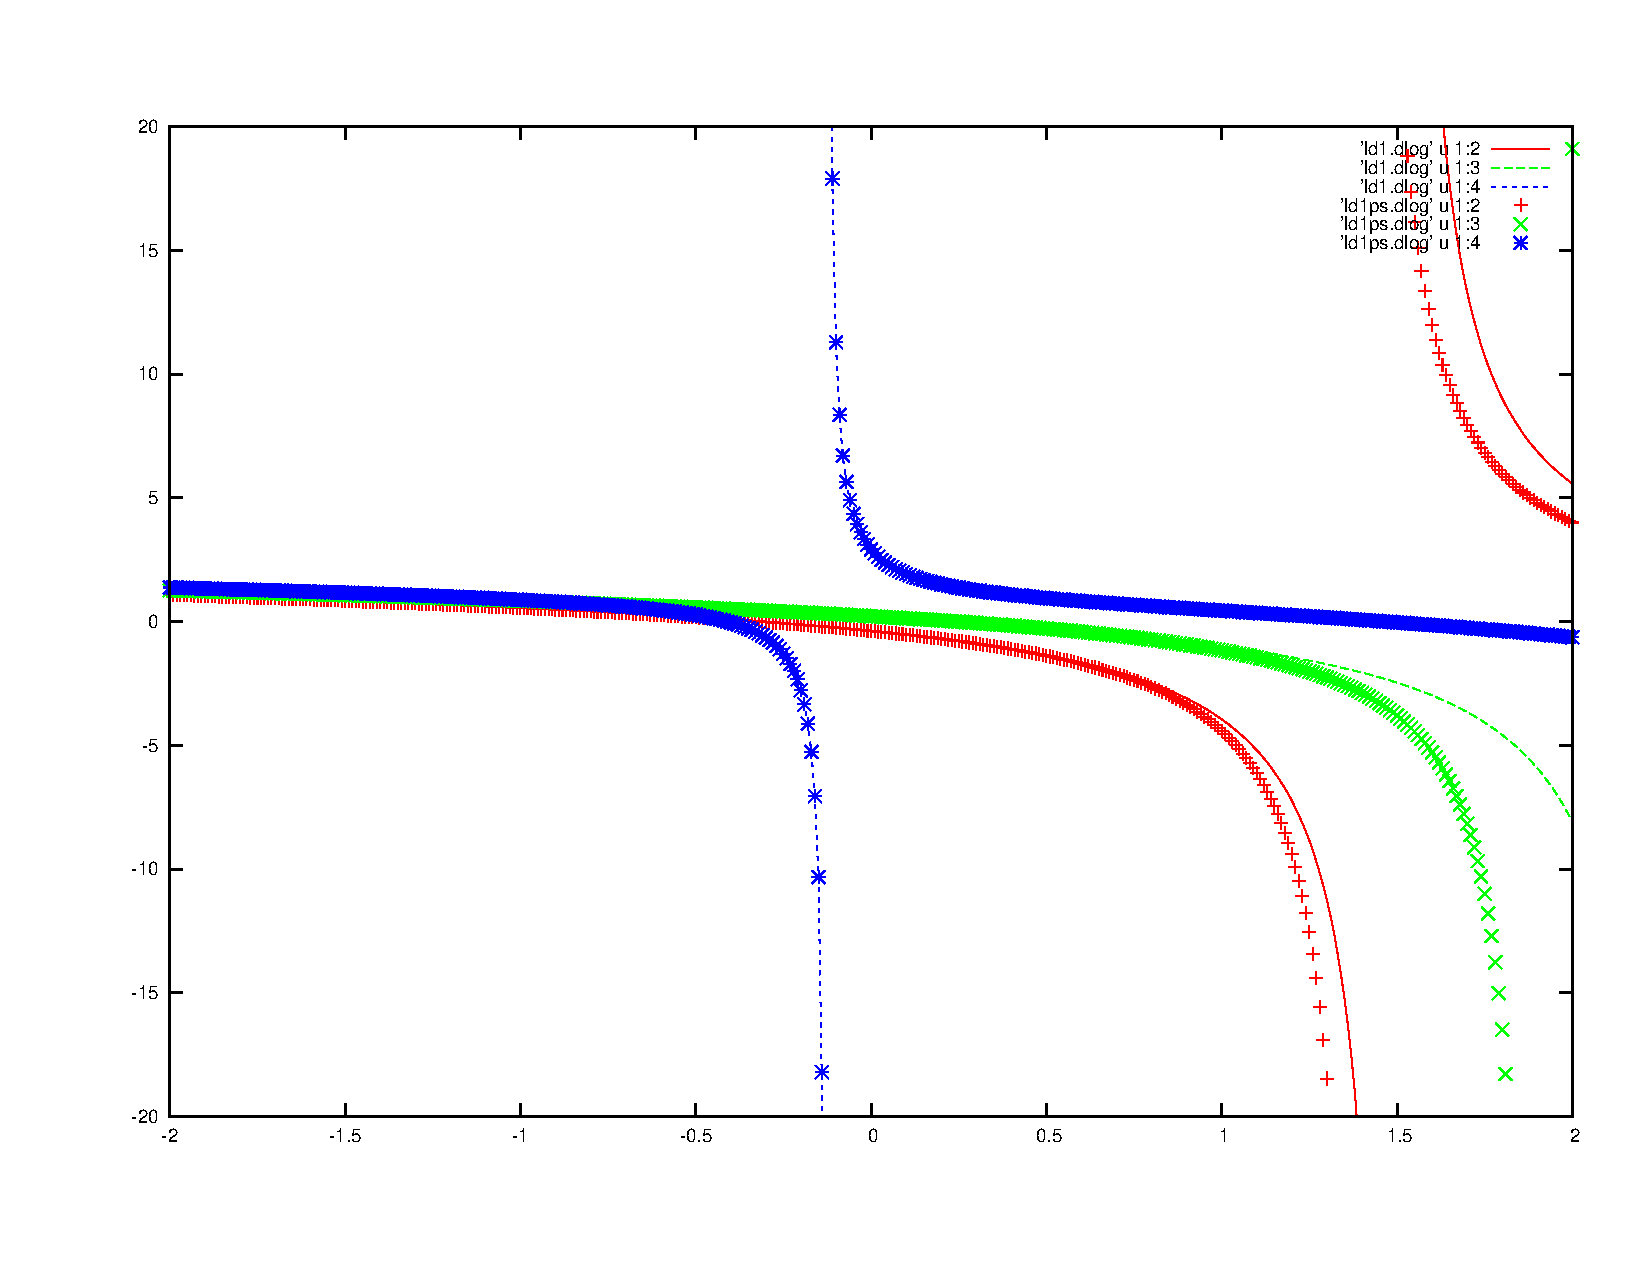
\includegraphics[width=7.5cm]{pseudo-gen-fig1.pdf}
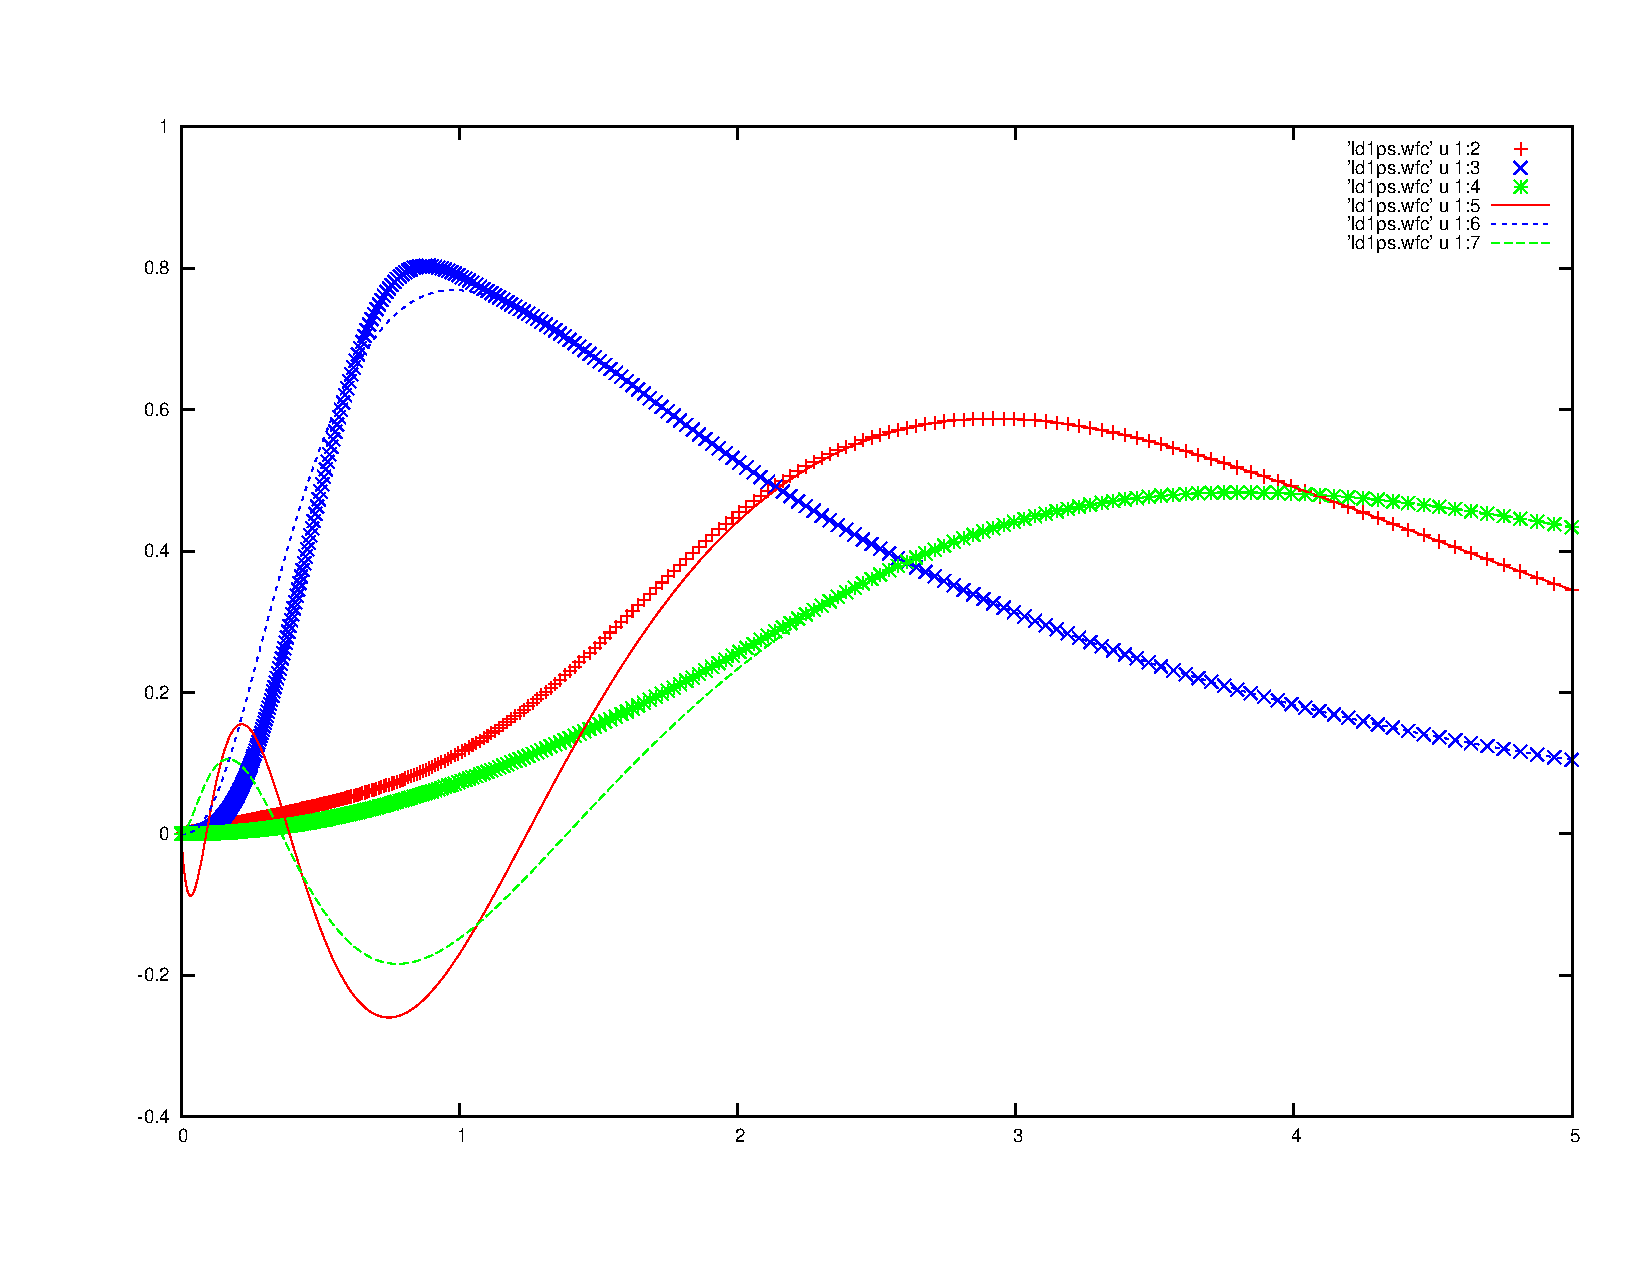
\includegraphics[width=7.5cm]{pseudo-gen-fig2.pdf}

We observe that our PP seems to reproduce fairly well
the logarithmic derivatives, with deviations appearing only at 
relatively high ($> 1$ Ry) energies. AE and PS orbitals match
very well beyond the pseudization radii; the $3d$ orbital is 
slightly deformed, because we have chosen a relatively large 
$r_c^{(l=2)}=1.3$ a.u.. It is easy to verify that a smaller
$r_c^{(l=2)}$ yields a better $3d$ PS orbital, but also a harder
$d$ potential: e.g., for $r_c^{(l=2)}=1.0$ a.u., you get
\begin{verbatim}
      Wfc   3D  rcut= 1.009  Estimated cut-off energy=      225.64 Ry
\end{verbatim}
Before proceding, it is wise to verify whether our PP has ``ghosts''.
Let us prepare the following input for the testing phase 
(note the variable \texttt{iswitch=2} and the \texttt{\&test}
namelist):
\begin{verbatim}
 &input
   atom='Ti',  dft='PBE',  config='[Ar] 3d2 4s2 4p0',
   iswitch=2
 /
 &test
   file_pseudo='Ti.pbe-rrkj.UPF',
   nconf=1, configts(1)='3d2 4s2 4p0',
   ecutmin=50, ecutmax=200, decut=50
 /
\end{verbatim}
This will solve the Kohn-Sham equation for the PP read from  
\texttt{file\_pseudo}, for a single valence configuration
(\texttt{nconf=1}) listed in \texttt{configts(1)} (the ground state
in this case), using a base of spherical waves whose cutoff
(in Ry) ranges from \texttt{ecutmin} to \texttt{ecutmax} in steps of
\texttt{decut}. The initial part of the output looks good, but let us
look at the test with spherical waves, towards the end:
\begin{verbatim}
     Cutoff (Ry) :  200.0
                          N = 1       N = 2       N = 3
     E(L=0) =        -0.7483 Ry   -0.3282 Ry   -0.0042 Ry
     E(L=1) =        -0.1077 Ry    0.0192 Ry    0.0630 Ry
     E(L=2) =        -0.2961 Ry    0.0304 Ry    0.0654 Ry
\end{verbatim}
The lowest levels found in this way should be the same\footnote{actually 
there are numerical differences, especially large for localized states 
like $3d$, whose origin is under investigation} 
as those calculated from radial integration (see above). 
This is true for the $4p$ state (-0.1077 Ry), 
for the $3d$ state (-0.2961 Ry vs -0.31302 Ry, see footnote),
for the $4s$ state (-0.3282 Ry)....but note the spurious $4s$ 
level at -0.7483 Ry! Our PP has a ghost and is unusable. 

What should be do now? we may try to change the definition of the
local potential. We had chosen $l=1$, let us try $l=2$ and $l=0$.
The former has the same pathology, the latter has no ghosts.
So our data for PP generation are as follows:
\begin{verbatim}
 &input
   atom='Ti',  dft='PBE',  config='[Ar] 3d2 4s2 4p0',
   rlderiv=2.90, eminld=-2.0, emaxld=2.0, deld=0.01, nld=3,
   iswitch=3
 /
 &inputp
   pseudotype=1, nlcc=.true., lloc=0,
   file_pseudopw='Ti.pbe-rrkj.UPF',
 /
3
4P 2 1 0.00  0.00 2.9 2.9
3D 3 2 2.00  0.00 1.3 1.3
4S 1 0 2.00  0.00 2.9 2.9
\end{verbatim}
(note \texttt{lloc=0} and the $4s$ state at the end of the list). 
Let us plot again logarithmic derivatives and orbitals (they look 
quite the same as before) and run again the test with spherical 
waves. We get (see the last section in the output):
\begin{verbatim}
     Cutoff (Ry) :   50.0
                           N = 1       N = 2       N = 3
     E(L=0) =        -0.3282 Ry   -0.0049 Ry    0.0361 Ry
     E(L=1) =        -0.1077 Ry    0.0192 Ry    0.0630 Ry
     E(L=2) =        -0.1469 Ry    0.0311 Ry    0.0682 Ry

     Cutoff (Ry) :  100.0
                           N = 1       N = 2       N = 3
     E(L=0) =        -0.3282 Ry   -0.0049 Ry    0.0361 Ry
     E(L=1) =        -0.1077 Ry    0.0192 Ry    0.0630 Ry
     E(L=2) =        -0.2959 Ry    0.0303 Ry    0.0652 Ry
     Cutoff (Ry) :  150.0
                           N = 1       N = 2       N = 3
     E(L=0) =        -0.3282 Ry   -0.0049 Ry    0.0361 Ry
     E(L=1) =        -0.1077 Ry    0.0192 Ry    0.0630 Ry
     E(L=2) =        -0.2961 Ry    0.0303 Ry    0.0652 Ry
\end{verbatim}
This time the first column yields (with a small discrepancy for $3d$)
the expected levels, and only those levels. It is wise to inspect
the second column as well for absence of suspiciously low levels: 
ghosts may appear also as spurious excited states close to occupied
states. Note how bad the energy for the $3d$ level is at 50 Ry.
At 100 Ry however we are close to convergence and at 150 Ry 
well converged, in agreement with the estimate given during 
the PP generation (138 Ry).

We have now our first candidate (i.e. not surely wrong) PP. 
In order to 1) verify if it really does the job, 2) quantify
its transferability, 3) quantify its hardness, and 4) improve 
it, if possible, we need to perform some more testing.

\subsubsection{Testing}

As a first idea of how good our PP is, let us verify how it
behaves on differente electronic configuration. The code
allows to test several configurations in the following way:
\begin{verbatim}
 &input
   atom='Ti',  dft='PBE',  config='[Ar] 3d2 4s2 4p0',
   iswitch=2
 /
 &test
   file_pseudo='Ti.pbe-rrkj.UPF',
   nconf=10
   configts(1)='3d2 4s2 4p0'
   configts(2)='3d2 4s1 4p1'
   configts(3)='3d2 4s1 4p0'
   configts(4)='3d2 4s0 4p0'
   configts(5)='3d3 4s1 4p0'
   configts(6)='3d1 4s2 4p1'
   configts(7)='3d1 4s2 4p0'
   configts(8)='3d1 4s1 4p0'
   configts(9)='3d1 4s0 4p0'
   configts(10)='3d0 4s0 4p0'
/
\end{verbatim}
here we have chosen 10 different valence configurations 
(the corresponding AE configurations are obtained by 
superimposing \texttt{configts} to core states in \texttt{config}).
Some of them are neutral, some are ionic, the first five leave
the $3d$ states unchanged, the last one is a completely ionized
Ti$^{4+}$. For each configuration, the code writes results 
(e.g. orbitals) into files \texttt{ld1}$N.*$ and \texttt{ld1ps}$N.*$,
where $N$ is the index of the configuration. A summary is written to
file \texttt{ld1.test}. For the first configuration, AE and PS 
eigenvalues and total energies are written:
\begin{verbatim}
     3 2     3D   1( 2.00)       -0.31302       -0.31302        0.00000
     1 0     4S   1( 2.00)       -0.32830       -0.32830        0.00000
     2 1     4P   1( 0.00)       -0.10777       -0.10777        0.00000
     Etot =   -1707.131006 Ry,    -853.565503 Ha,  -23226.698556 eV
     Etotps =    -9.748745 Ry,      -4.874372 Ha,    -132.638416 eV
\end{verbatim}
(AE and PS eigenvalues are in this case the same, since this is the
reference configuration used to build the PP). For the following
configurations, AE and PS eigenvalues, plus total energy
{\em differences}\footnote{Reminder: absolute PS total energies 
depend upon the specific PP! Only energy differences are significant.}
wrt configuration 1 are printed:
\begin{verbatim}
     3 2     3D   1( 2.00)       -0.40319       -0.40457        0.00138
     1 0     4S   1( 1.00)       -0.38394       -0.38420        0.00026
     2 1     4P   1( 1.00)       -0.15248       -0.15237       -0.00011
     dEtot_ae =       0.226061 Ry
     dEtot_ps =       0.226250 Ry,   Delta E=      -0.000189 Ry
\end{verbatim}
The discrepancy between AE and PS energy differences (in this case,
wrt the ground state) as well as the discrepancies in AE and PS 
eigenvalues, are a measure of how transferrable a PP is. In this case,
the AE-PS discrepancy on $\delta E = E(4s^14p^13d^2) - E(4s^24p^03d^2)$
(look at \texttt{Delta E}) is quite small, $<0.2$ mRy, while the 
maximum discrepancy of the eigenvalues (rightmost column) $\sim 1$ mRy. 
These are very good results.
Unfortunately this is also a configuration that doesn't differ much
from the reference one. Let us see the other cases:
\begin{verbatim}
     3 2     3D   1( 2.00)       -0.83550       -0.83256       -0.00295
     1 0     4S   1( 1.00)       -0.76075       -0.76163        0.00088
     2 1     4P   1( 0.00)       -0.48549       -0.48617        0.00068
     dEtot_ae =       0.539968 Ry
     dEtot_ps =       0.540344 Ry,   Delta E=      -0.000376 Ry
 
     3 2     3D   1( 2.00)       -1.44648       -1.44538       -0.00110
     1 0     4S   1( 0.00)       -1.24186       -1.24652        0.00465
     2 1     4P   1( 0.00)       -0.91224       -0.91599        0.00375
     dEtot_ae =       1.537516 Ry
     dEtot_ps =       1.540285 Ry,   Delta E=      -0.002769 Ry
 
     3 2     3D   1( 3.00)       -0.14077       -0.12814       -0.01263
     1 0     4S   1( 1.00)       -0.27408       -0.28302        0.00894
     2 1     4P   1( 0.00)       -0.08212       -0.08867        0.00655
     dEtot_ae =       0.081274 Ry
     dEtot_ps =       0.095152 Ry,   Delta E=      -0.013878 Ry
 
     3 2     3D   1( 1.00)       -0.68514       -0.74236        0.05722
     1 0     4S   1( 2.00)       -0.45729       -0.45802        0.00073
     2 1     4P   1( 1.00)       -0.18855       -0.18471       -0.00383
     dEtot_ae =       0.343391 Ry
     dEtot_ps =       0.371650 Ry,   Delta E=      -0.028259 Ry
 
     3 2     3D   1( 1.00)       -1.16621       -1.21438        0.04817
     1 0     4S   1( 2.00)       -0.87720       -0.87620       -0.00100
     2 1     4P   1( 0.00)       -0.56807       -0.56137       -0.00670
     dEtot_ae =       0.716203 Ry
     dEtot_ps =       0.739110 Ry,   Delta E=      -0.022907 Ry
 
     3 2     3D   1( 1.00)       -1.82248       -1.87471        0.05223
     1 0     4S   1( 1.00)       -1.39447       -1.39936        0.00489
     2 1     4P   1( 0.00)       -1.03942       -1.03465       -0.00476
     dEtot_ae =       1.848995 Ry
     dEtot_ps =       1.873240 Ry,   Delta E=      -0.024245 Ry
 
     3 2     3D   1( 1.00)       -2.54976       -2.61959        0.06983
     1 0     4S   1( 0.00)       -1.94361       -1.96745        0.02383
     2 1     4P   1( 0.00)       -1.53584       -1.54419        0.00835
     dEtot_ae =       3.518170 Ry
     dEtot_ps =       3.554733 Ry,   Delta E=      -0.036564 Ry
 
     3 2     3D   1( 0.00)       -3.84145       -3.95251        0.11106
     1 0     4S   1( 0.00)       -2.73793       -2.81405        0.07612
     2 1     4P   1( 0.00)       -2.25938       -2.28768        0.02831
     dEtot_ae =       6.699594 Ry
     dEtot_ps =       6.831938 Ry,   Delta E=      -0.132344 Ry
\end{verbatim} 
It is evident that configurations with $3d^2$ occupancy are well 
reproduced, with errors on total energy differences $<3$ mRy and
on eigenvalues$<5$ mRy. Configurations with different $3d$ occupancy,
however, have errors one order of magnitude higher. For the extreme
case of Ti$^{4+}$, the error is $\sim$ 0.1 Ry.

\newpage



\appendix

\section{Atomic Calculations}

\subsection{Nonrelativistic case}

Let us assume that the charge density $n(r)$ and the potential $V(r)$
are spherically symmetric. The Kohn-Sham (KS) equation:
\begin{equation}
\left(-{\hbar^2\over 2m}\nabla^2 + V(r)-\epsilon\right) \psi(\r)=0
\end{equation}
can be written in spherical coordinates. We write the wavefunctions as
\begin{equation}
\psi(\r)=\left({R_{nl}(r)\over r}\right)Y_{lm}(\hat\r),
\end{equation}
where $n$ is the main quantum 
number $l=n-1,n-2,\dots,0$ is angular momentum, $m=l,l-1,\dots,-l+1,-l$
is the projection of the angular momentum on some axis. 
The radial KS equation becomes:
\begin{eqnarray}
\left(-{\hbar^2\over 2m} {1\over r} {d^2 R_{nl}(r)\over dr^2}
      +(V(r)-\epsilon) {1\over r} R_{nl}(r)
\right) Y_{lm}(\hat\r) \hskip 4cm \nonumber \\ \mbox{} - 
{\hbar^2\over 2m} \left({1\over\mbox{sin}\theta}{\partial\over\partial\theta}
                        \left(\mbox{sin}\theta{\partial Y_{lm}(\hat\r)
                                               \over\partial\theta}\right)
                      + {1\over\mbox{sin}^2\theta}
                           {\partial^2Y_{lm}(\hat\r)\over\partial\phi^2}
                  \right) {1\over r^3} R_{nl}(r) = 0.
\end{eqnarray}
This yields an angular equation for the spherical harmonics $Y_{lm}(\hat\r)$:
\begin{equation}
-\left({1\over\mbox{sin}\theta}{\partial\over\partial\theta}
       \left(\mbox{sin}\theta{\partial Y_{lm}(\hat\r)\over\partial\theta}
       \right)
     + {1\over\mbox{sin}^2\theta}
                           {\partial^2Y_{lm}(\hat\r)\over\partial\phi^2}
\right) = l(l+1)Y_{lm}(\hat\r)
\end{equation}
and a radial equation for the radial part $R_{nl}(r)$:
\begin{equation}
-{\hbar^2\over 2m} {d^2 R_{nl}(r)\over dr^2}
+\left( {\hbar^2\over 2m} {l(l+1)\over r^2} + V(r)-\epsilon
\right) R_{nl}(r) = 0.
\end{equation}
The charge density is given by
\begin{equation}
n(r) = \sum_{nlm} \Theta_{nl}\left |{R_{nl}(r)\over r}Y_{lm}(\hat r)\right|^2 
     = \sum_{nl} \Theta_{nl}{R^2_{nl}(r)\over 4\pi r^2}
\end{equation}
where $\Theta_{nl}$ are the occupancies ($\Theta_{nl}\le 2l+1$)
and it is assumed that the occupancies of $m$ are such as to yield
a spherically symmetric charge density (which is true only for closed
shell atoms).
\subsubsection{Useful formulae} 

Gradient in spherical coordinates $(r,\theta,\phi)$:
\begin{equation}
\nabla\psi = \left({\partial\psi\over\partial r},
                   {1\over r}{\partial\psi\over\partial\theta},
                   {1\over r \mbox{sin}\theta}
                              {\partial\psi\over\partial\phi}
             \right)
\end{equation}
Laplacian in spherical coordinates:
\begin{equation}
\nabla^2\psi = {1\over r} {\partial^2\over\partial r^2}(r\psi)
             + {1\over r^2\mbox{sin}\theta} {\partial\over\partial\theta}
               \left(\mbox{sin}\theta{\partial\psi\over\partial\theta}\right)
             + {1\over r^2\mbox{sin}^2\theta}
                {\partial^2\psi\over\partial\phi^2}
\end{equation}

\subsection{Fully relativistic case} 

The relativistic KS equations are
Dirac-like equations for a spinor with a ``large'' $R_{nlj}(r)$ and
a ``small'' $S_{nlj}(r)$ component:
\begin{eqnarray}
c\left({d \over dr} + {\kappa\over r}\right)R_{nlj}(r) & = & 
       \left(2mc^2 - V(r) + \epsilon \right)S_{nlj}(r)\\
c\left({d \over dr} - {\kappa\over r}\right)S_{nlj}(r) & = & 
       \left( V(r) + \epsilon \right)       R_{nlj}(r)
\end{eqnarray}
where $j$ is the total angular momentum ($j=1/2$ if $l=0$, 
$j=l+1/2,l-1/2$ otherwise); $\kappa=-2(j-l)(j+1/2)$ is the Dirac 
quantum number ($\kappa=-1$ is $l=0$, $\kappa=-l-1,l$ otherwise);
and the charge density is given by
\begin{equation}
  n(r) = \sum_{nlj} \Theta_{nlj}{R^2_{nlj}(r)+S^2_{nlj}(r)\over 4\pi r^2}.
\end{equation}


\subsection{Scalar-relativistic case} 

The full relativistic KS equations
is be transformed into an equation for the large component only
and averaged over spin-orbit components. In atomic units
(Rydberg: $\hbar=1, m=1/2, e^2=2$):
\begin{eqnarray}
-{d^2 R_{nl}(r)\over dr^2}
+\left( {l(l+1)\over r^2} + M(r)\left(V(r)-\epsilon\right)
\right) R_{nl}(r) \qquad \nonumber \\ \mbox{} -
 {\alpha^2\over 4M(r)} {dV(r)\over dr} 
                    \left({dR_{nl}(r)\over dr} +
                          \langle\kappa\rangle {R_{nl}(r)\over r}\right)= 0,
\end{eqnarray}
where $\alpha=1/137.036$ is the fine-structure constant,
$\langle\kappa\rangle=-1$ is the degeneracy-weighted average value 
of the Dirac's $\kappa$ for the two spin-orbit-split levels, $M(r)$ is
defined as
\begin{equation}
M(r)= 1 - {\alpha^2\over 4} \left(V(r)-\epsilon\right).
\end{equation}
The charge density is defined as in the nonrelativistic case:
\begin{equation}
n(r) = \sum_{nl} \Theta_{nl}{R^2_{nl}(r)\over 4\pi r^2}.
\end{equation}

\subsection{Numerical solution} 

The radial (scalar-relativistic) KS equation is integrated 
on a radial grid. It is convenient to
have a denser grid close to the nucleus and a coarser one far
away. Traditionally a logarithmic grid is used: 
$r_i=r_0\mbox{exp}(i\Delta x)$. With this grid, one has
\begin{equation}
\int_0^\infty f(r) d r = \int_0^\infty f(x) r(x) dx
\end{equation}
and
\begin{equation}
{d f(r)\over d r}={1\over r} {d f(x)\over d x},\qquad
{d^2 f(r)\over d r^2}=-{1\over r^2} {d f(x)\over d x}
+ {1\over r^2} {d^2 f(x)\over d x^2}.
\end{equation}
We start with a given self-consistent potential $V$ and
a trial eigenvalue $\epsilon$. The equation is integrated
from $r=0$ outwards to $r_t$, the outermost classical 
(nonrelativistic for simplicity) turning point, defined
by $ {l(l+1) /r_t^2} + \left(V(r_t)-\epsilon\right)=0$.
In a logarithmic grid (see above) the equation to solve becomes:
\begin{eqnarray}
{1\over r^2} {d^2 R_{nl}(x)\over d x^2} & = & 
  {1\over r^2} {d R_{nl}(x)\over d x} + 
  \left( {l(l+1)\over r^2} + 
  M(r)\left(V(r)-\epsilon\right) \right) R_{nl}(r) \nonumber \\
 & & \mbox{} - {\alpha^2\over 4M(r)} {dV(r)\over dr} 
      \left({1\over r} {dR_{nl}(x)\over dx} +
            \langle\kappa\rangle {R_{nl}(r)\over r}\right).
\end{eqnarray}
This determines ${d^2 R_{nl}(x)/d x^2}$ which is used to
determine ${d R_{nl}(x)/ dx}$ which in turn is used to
determine $R_{nl}(r)$, using predictor-corrector or whatever
classical integration method. ${dV(r)/dr}$ is evaluated
numerically from any finite difference method. The series
is started using the known (?) asymptotic behavior of $R_{nl}(r)$ 
close to the nucleus (with ionic charge $Z$)
\begin{equation}
R_{nl}(r)\simeq r^\gamma,\qquad \gamma={l\sqrt{l^2-\alpha^2 Z^2}+
(l+1)\sqrt{(l+1)^2-\alpha^2 Z^2}\over 2l+1}.
\end{equation}
The number of nodes is counted. If there are too few (many)
nodes, the trial eigenvalue is increased (decreased) and
the procedure is restarted until the correct number $n-l-1$
of nodes is reached. Then a second integration is started 
inward, starting from a suitably large $r\sim 10r_t$ down 
to $r_t$, using as a starting point the asymptotic behavior 
of $R_{nl}(r)$ at large $r$: 
\begin{equation}
R_{nl}(r)\simeq e^{-k(r)r},\qquad 
k(r)=\sqrt{{l(l+1)\over r^2} + \left(V(r)-\epsilon\right)}.
\end{equation}
The two pieces are continuously joined at $r_t$ and a correction to the trial 
eigenvalue is estimated using perturbation theory (see below). The procedure 
is iterated to self-consistency.

The perturbative estimate of correction to trial eigenvalues is described in
the following for the nonrelativistic case (it is not worth to make relativistic
corrections on top of a correction). The trial eigenvector $R_{nl}(r)$ will have 
a cusp at $r_t$ if the trial eigenvalue is not a true eigenvalue:
\begin{equation}
A = {d R_{nl}(r_t^+)\over dr} - {d R_{nl}(r_t^-)\over dr} \ne 0.
\end{equation}
Such discontinuity in the first derivative translates into a
$\delta(r_t)$ in the second derivative:
\begin{equation}
{d^2  R_{nl}(r)\over dr^2} = {d^2 \widetilde R_{nl}(r)\over dr^2}
  + A \delta(r-r_t)
\end{equation}
where the tilde denotes the function obtained by matching the
second derivatives in the $r< r_t$ and $r> r_t$ regions.
This means that we are actually solving a different problem in which 
$V(r)$ is replaced by $V(r)+\Delta V(r)$, 
given by
\begin{equation}
 \Delta V(r) = -{\hbar^2 \over 2m} {A\over R_{nl}(r_t)}\delta(r-r_t).
\end{equation}
The energy difference between the solution to such fictitious potential 
and the solution to the real potential can be estimated from
perturbation theory:
\begin{equation}
 \Delta\epsilon_{nl} = - \langle\psi|\Delta V |\psi\rangle
                     =   {\hbar^2 \over 2m} R_{nl}(r_t) A.
\end{equation}

\section{Equations for the Troullier-Martins method}

We assume a pseudowavefunction $R^{ps}$ having the following form:
\begin{eqnarray}
R^{ps}(r)&=&r^{l+1}e^{p(r)} \quad r\le r_c \\
R^{ps}(r)&=&R(r)         \quad r\ge r_c
\end{eqnarray}
where
\begin{equation}
p(r)=c_0+c_2r^2+c_4r^4+c_6r^6+c_8r^8+c_{10}r^{10}+c_{12}r^{12}.
\end{equation}
On this pseudowavefunction we impose the norm conservation
condition:
\begin{equation}
\int_{r<r_c} (R^{ps}(r))^2 dr=\int_{r<r_c} (R(r))^2 dr
\end{equation}
and continuity conditions on the wavefunction and its derivatives up
to order four at the matching point:
\begin{equation}
{d^nR^{ps}(r_c)\over dr^n}={d^nR(r_c)\over dr^n}, \quad n=0,...,4
\end{equation}

\noindent$\bullet$ Continuity of the wavefunction:
\begin{equation}
R^{ps}(r_c)=r_c^{l+1}e^{p(r_c)}=R(r_c)
\end{equation}
\begin{equation}
p(r_c) = \mbox{log}{R(r_c)\over r_c^{l+1}} 
\end{equation}

\noindent$\bullet$ Continuity of the first derivative of the wavefunction:
\begin{equation}
{dR^{ps}(r)\over dr} = (l+1)r^le^{p(r)} + r^{l+1}e^{p(r)}p'(r)
                         ={l+1\over r}R^{ps}(r) + p'(r)R^{ps}(r)
\end{equation}
that is
\begin{equation}
 p'(r_c) = {dR(r_c)\over dr} {1\over R^{ps}(r_c)} -
           {l+1\over r_c}.
\end{equation}

\noindent$\bullet$ Continuity of the second  derivative of the wavefunction:
\begin{eqnarray}
{d^2R^{ps}(r)\over d^2r} 
   & = &
     {d\over dr}\left((l+1)r^le^{p(r)} + r^{l+1}e^{p(r)}p'(r)\right) 
\nonumber \\ & = &
     l(l+1)r^{l-1}e^{p(r)} + 2(l+1)r^le^{p(r)}p'(r) +
     r^{l+1}e^{p(r)}\left[p'(r)\right]^2 + r^{l+1}e^{p(r)}p''(r)
\nonumber\\ & = &
     \left( {l(l+1)\over r^2}+ {2(l+1)\over r}p'(r) +
            \left[p'(r)\right]^2 + p''(r) \right) r^{l+1}e^{p(r)}.
\end{eqnarray}
From the radial Schr\"odinger equation:
\begin{equation}
 {d^2R^{ps}(r)\over dr^2} = 
    \left ( {l(l+1)\over r^2} +{2m\over\hbar^2}(V(r)-\epsilon)\right)R^{ps}(r)
\end{equation}
that is
\begin{equation}
p''(r_c) = {2m\over\hbar^2}(V(r_c)-\epsilon) - 2 {l+1\over r_c}p'(r_c)
         -\left[p'(r_c)\right]^2 
\end{equation}

\noindent$\bullet$ Continuity of the third and fourth derivatives of the
wavefunction. This is assured if the third and fourth derivatives of
$p(r)$ are continuous. By direct derivation of the expression of
$p''(r)$:
\begin{equation}
p'''(r_c) = {2m\over\hbar^2}V'(r_c) + 2 {l+1\over r^2_c}p'(r_c)
          - 2{l+1\over r_c}p''(r_c) -2 p'(r_c)p''(r_c)
\end{equation}

\begin{eqnarray}
p''''(r_c) & = & {2m\over\hbar^2}V''(r_c) - 4 {l+1\over r^3_c}p'(r_c)
                 + 4{l+1\over r^2_c}p''(r) \nonumber \\ & & \mbox{} 
            - 2{l+1\over r_c}p'''(r_c)
           - 2 \left[p''(r_c)p''(r_c)\right]^2 -2 p'(r_c)p'''(r_c)
\end{eqnarray}

The additional condition: $V''(0)=0$ is imposed. 
The screened potential is
\begin{eqnarray}
V(r)&=&{\hbar^2\over2m}\left({1\over R^{ps}(r)}{d^2R^{ps}(r)\over dr^2} 
     - {l(l+1)\over r^2}\right)+\epsilon \\
    &=&{\hbar^2\over2m}\left( 2{l+1\over r} p'(r)+\left[p(r)\right]^2+p''(r)
       \right)+\epsilon
\end{eqnarray}

Keeping only lower-order terms in $r$:
\begin{eqnarray}
V(r) &\simeq&{\hbar^2\over2m}\left( 2{l+1\over r} (2c_2r + 4c_4r^3) 
               + 4c_2^2r^2 + 2c_2 + 12c_4r^2\right) + \epsilon \\
     &   =  & {\hbar^2\over2m}\left( 2c_2(2l+3) + 
              \left((2l+5)c_4+c_2^2\right) r^2\right)+ \epsilon .
\end{eqnarray}
The additional constraint is:
\begin{equation}
(2l+5)c_4+c_2^2=0.
\end{equation}



\begin{thebibliography}{10}

\bibitem{NC} 
D.R. Hamann, M. Schl\"uter, and C. Chiang, 
Phys. Rev. Lett. {\bf 43}, 1494 (1979).

\bibitem{van} D. Vanderbilt, Phys. Rev. B  {\bf 47}, 10142 (1993).

\bibitem{PAW} P.~E. Bl\"ochl, Phys. Rev. B {\bf 50}, 17953 (1994).

\bibitem{BHS} 
G.B. Bachelet, D.R. Hamann and M. Schl\"uter, Phys. Rev. B {\bf 26},
4199 (1982). 

\bibitem{Gonze} 
X. Gonze, R. Stumpf, and M. Scheffler, Phys. Rev. B {\bf 44}, 8503 (1991).

\bibitem{Goedecker} 
S. Goedecker, M. Teter, and J. Hutter, Phys. Rev. B {\bf 54}, 1703 (1996).

\bibitem{TM} N. Troullier and J.L. Martins, Phys. Rev. B {\bf 43},
1993 (1991).

\bibitem{fhi98PP} 
M.Fuchs and M. Scheffler, Comput. Phys. Commun. {\bf 119}, 67 (1999).

\bibitem{RRKJ} A. M. Rappe, K. M. Rabe, E. Kaxiras, and J. D. Joannopoulos, 
Phys. Rev. B {\bf 41}, 1227 (1990) 
(erratum: Phys. Rev. B {\bf 44}, 13175 (1991)).

\bibitem{KB} L. Kleinman and D.M. Bylander, Phys. Rev. Lett. 48, 1425 (1982).

\bibitem{CoreCorr} 
S.G. Louie, S. Froyen, and M.L. Cohen, Phys. Rev. B {\bf 26}, 1738 (1982).

\bibitem{Zunger} S.H. Wei and A. Zunger, Phys. Rev. B {\bf 37}, 8958 (1987).

\end{thebibliography}

\end{document}
